
\documentclass[11pt,conference]{IEEEtran} 
%\documentclass[conference]{IEEEtran}
\usepackage{cite}
\usepackage[pdftex]{graphicx}
\usepackage[cmex10]{amsmath}
\usepackage{algorithmic}
\usepackage[tight,footnotesize]{subfigure}
\usepackage{url}
\usepackage{algorithm2e}
\usepackage{verbatim}

\begin{document}

% paper title
% can use linebreaks \\ within to get better formatting as desired
\title{Fair Energy Consumption in Wireless Sensor Networks}
% author names and affiliations
% use a multiple column layout for up to three different
% affiliations
\author{\IEEEauthorblockN{Niels Kasch*}
\IEEEauthorblockA{Email: nkasch1@umbc.edu}
\and
\IEEEauthorblockN{Dave Feltenberger*}
\IEEEauthorblockA{Email: dfelten1@umbc.edu\\\\
*Department of Computer Science and\\Electrical Engineering\\
University of Maryland, Baltimore County\\
Baltimore, MD 21250\\
April 27$^{\textrm{th}}$, 2009\\
}
\and
\IEEEauthorblockN{Fatih Senel*}
\IEEEauthorblockA{Email: fsenel1@umbc.edu}
}

\maketitle



\begin{abstract}
We introduce the notion of \textit{fairness} in power consumption of wireless sensor networks (WSNs). 
Herein, \textit{fairness} in power consumption refers to an approximately equal power consumption rate among all nodes in a WSN. This topic has been largely overlooked by the literature, but has a significant impact in the design of WSNs with fixed sensor nodes and resource scarce flexible relay nodes.

We propose an approximation algorithm with the aim to introduce fairness to power consumption in WSNs. While overall power consumption has been studied previously, our algorithm considers fairness of power consumption rates a priority in WSN design. Our algorithm introduces additional, limited resources (i.e. relay nodes) to a fixed network. These resources may be moved to achieve minimal overall power consumption and maximum fairness. Hence, we give a multi-objective optimization algorithm for (1) maximum fairness in power consumption, (2) minimal additional resources and (3) minimal power consumption of WSNs.

Experimental analysis of randomly generated WSNs show that the introduction of a small numbers of relay nodes (as compared to sensor nodes) results in a significant increase in fairness of power consumption. However, as further relay nodes are added, we encounter a diminishing return in the increase of fairness. Hence, we pose the question of optimality considering the trade off between fairness and relay nodes and give a discussion for the experimental determination of such optimality.

We briefly illustrate our WSN fairness simulation software that utilizes the algorithm and visualizes the process of optimizing a WSN for fairness.
\end{abstract}

\begin{keywords}
Wireless Sensor Network, Energy Conservation, Fairness, Energy Consumption
\end{keywords}

\IEEEpeerreviewmaketitle


\section{Introduction}

Over the past decade, research in the area of Wireless Sensor Networks (WSN) has produced valuable insight in the private, public and medical sectors. WSNs consist of a collection of independent devices (nodes) that are connected wirelessly in an ad hoc fashion. Generally, each node is equipped with sensors collecting information from and monitoring its environment. Evaluation of such information enables reactive, proactive and modeling capabilities each of which is utilized in fields such as traffic control, home automation and biomedication, to name a few.

The size of WSNs ranges from a few nodes to upwards of 10000 nodes covering areas beyond wireless transmission capabilities. Multi-hop networking is an integral part in these networks to ensure connectivity between all nodes. Connectivity is by far the most important criterion involved in WSN design decisions. Extensive research has been conducted to:
\begin{itemize}
\item identify ways to interconnect all nodes with a minimum number of links. The Minimum Spanning Tree (MST) adopted from graph theory and general networking addresses this issue.
\item interconnect nodes by a network of shortest length when additional nodes (i.e. relay nodes) are introduced. This problem has been studied as the Steiner Tree problem.
\item optimize a network of shortest length according to a restricting parameter. In WSN, the transmission range of a node may impose limits on the length of a link.
\end{itemize}

A second important criterion, which is the focus of our work, is the energy efficiency of the network. Nodes in a WSN are typically battery powered and as such their lifetime can be measured by their average battery lifetime. In medical applications such as patient embedded sensors, battery conservation becomes a matter involving the quality of life for a patient. The shorter the lifetime of a sensor node, the more often a patient must undergo node replacement procedures. 

Wireless radio transmissions drop off at an exponential rate due to ground reflection of radio signals. The further a signal should travel to more energy must be utilized. Since the signal attenuation rate is exponential with distance, a significant amount of energy must be used to transmit a signal only a small distance further. Chang et. al \cite{RelaySensor} investigated WSN power consumption optimization by imposing a global maximum transmission range and employing Steiner Points in the resulting Steiner Minimum Tree as relay nodes to ensure connectivity. Using this technique, \cite{RelaySensor} were able to conserve a significant amount of energy in the overall WSN topology.

While overall power consumption is certainly an improvement over previous architectures, we are interested in identifying approximately equal power consumption for every node in the network. Our work would have an important impact on WSN where predictability of equal power consumptions is important. For example, if the battery lifetime of every node in a WSN for patient biomedication is approximately equal and maximized, then a patient will undergo the fewest number of  node replacement procedures. During such a procedure, every node can be replaced as battery lifetimes are approximately equal. This idea differs from previous work in that power consumption of the network as a whole is equalized and optimized as opposed to only optimizing the power consumption which may leave individual nodes with differing power consumption rates. Hence, we introduce the notion of \textit{fairness} of power consumption in WSN. We, therefore, propose a two-fold optimization problem as follows:
Optimize the fairness of a measure $F_n$ for each node $n$ across a wireless sensor network, given that $F_n$ is exponentially related to a distance measure between neighboring nodes. Thus, $F_n$ is to be minimized. Furthermore, the network is to be connected in a way such that, after the addition of a minimal number of relay nodes, the spanning tree connecting the network is of minimum length and the distances between nodes are approximately equal.

\subsection{Problem Formulation}
Specifies the problem (i.e. fairness in WSN) we are addressing in this paper. Defines the key concepts, such a fairness in relation to power consumption and efficiency of power consumption as well as addresses pitfalls such as minimal power consumption which is not addressed by this paper.
\subsection{System Model}
The system model is explained. All assumptions required for the model are specified.

Important performance metrics, such as:
\begin{itemize}
\item \texttt{time to death of the first node}(TTFD)
\item \texttt{average node lifetime} (ANL)
\item \texttt{cut vertex lifetime} and its optimality
\item additional resource requirements such as \texttt{number of Steiner points} and additional nodes
\item $L$ - maximum power consumption rate
\item $K$ - number of new Steiner Points
\item $\alpha$ - minimum standard deviation of power consumption rates given $K$ Steiner points
\end{itemize}
are defined in this section.
\section{Related Work}

Cheng \cite{RelaySensor} proposed a relay node placement algorithm using the minimum number of relay nodes, so that the distance between each hop is less than or equal to the common transmission range. This problem is similar to the Steiner Minimum Tree with minimum number of Steiner Points and bounded edge-length (SMT-MSPBEL). They proposed a 3-approximation algorithm and a 2.5 approximation algorithm. The 2.5 approximation algorithm is a randomized algorithm whose performance is faster than 3-approximation algorithm.

Lloyd \cite{1191701} discusses two strategies for ensuring a WSN is fully connected.  The first is a single-tiered node placement strategy in which every node is connected via some path consisting of either sensor nodes or relay nodes.  The length between a sensor node and any other node must be <= r, while the length between two relay nodes can be of distance R, where R is defined as R >= r.  Node placement is achieved using Steiner Tree nodes.

The second strategy discussed is what they call a two-tiered node placement strategy, in which any two nodes of the WSN are fully connected by all relay nodes. That is, between any two sensor nodes in the WSN there exists a path by which every intermediary node is a relay node.

Recent research on relay node placement in Wireless Sensor Networks mostly focuses on connectivity establishment (Estrin et al. \cite{940390}). Connectivity is one of the most crucial issue, since most of the actions are taken collaboratively. In addition, sensors are small battery operated devices. Usually after the deployment of wireless sensor networks, it is impossible to access a sensor node and change the battery. Once the battery is depleted the node dies. The most important source of energy consumption in sensor networks is message transmission. The energy required to transmit data is directly proportional to $r^4$ where $r$ is the distance between source and destination.

NEED TO REFER TO THIS PAPER\cite{596303}.
\section{Proposed Approach}\label{approach}

\subsection{System Model}
The model and algorithms described in this paper make the following assumptions:

\begin{itemize}
\item Each sensor/node sends an equal amount of data per time unit.
\item Each node can receive an arbitrary amount of data per time unit.
\item Each node can store an arbitrary amount of data without energy penalties. This assumption enables this model to ignore data transmission bottlenecks.
\item The transmission range of each sensor node does not exceed the maximum transmission range $T$.
\item Only nodes within transmission range of each other are connected (i.e. have an edge between each other in the network).
\item A node's energy dissipation per bit transmitted (according to the first order radio model \cite{820485}).
\item Transmitting a bit over distance $d$ requires energy $d^2$.
\item Sensor nodes have a fixed location. Their location may not change during the lifetime of the network.
\item Relay nodes are movable. Their location is flexible during the lifetime of the network.
\item Relay nodes can be added to the original network.
\end{itemize}

\subsection{Problem Formulation}

In the Minimal Fair Energy Consumption with Minimal Additional Resources (MFEC-MAR) problem the goal, given a wireless sensor network represented as a graph $G=(V \cup S,E)$, is to equalize the power consumption rate $PCR$ of all nodes in $G$. That is $PCR(v_1)=PCR(v_2)=PCR(v_3)=...=PCR(v_n)$ where $n=|V \cup S|$ denotes the number of vertices/nodes in $G$. The set of vertices in $G$ is composed of a set of fixed vertices $V$ (i.e. sensor nodes) and a set of moveable vertices $S$ (i.e. relay nodes). The edges $E$ in $G$ are subject to the maximum transmission range $T$ of the nodes. It is furthermore the goal of MFEC-MAR to minimize overall power consumption of the network such that $\sum_{i=1}^{n} PCR(v_i)$ is minimal. The set of moveable vertices $S$ is adjustable in $|S|$ and is minimized as well. Hence, MFEC-MAR is a multi-objective optimization problem (MOP). Formally, MFEC-MAR is defined as follows:

\begin{itemize}
 \item \textbf{Input:} A sensor network $G = (V, E)$, where $V$ is a set of fixed vertices and $E$ is the set of edges between vertices if they are within transmission range $T$, a fairness measure $\alpha$, a maximum power consumption rate $P$

\item \textbf{Output:} A non-disconnected network $G' = (V \cup S, E')$ such that:
	\begin{itemize}
		\item $STDEV( PCR_{v \in |V \cup S|} v) \leq \alpha$
		\item $\forall_{v \in |V \cup S|} PCR(v) \leq P$
		\item $\sum_{v \in |V \cup S|} PCR(v)$ is minimal
		\item $|S|$ is minimal
	\end{itemize}
\end{itemize}

For the remainder of this paper, whenever we refer to fairness of power consumption rates ($PCR$), we denote this fairness measure $\alpha$ as the maximum allowable standard deviation of power consumption rates.


\subsection{Algorithms for MFEC-MAR (Fairness in WSNs)}
In this section we will explain our two step approach to solving the fairness problem in WSNs.

\subsubsection{Connecting Nodes}
This section explains how to connect and initially disconnected set of nodes using the Steiner Minimum Tree (SMT) algorithm.
\subsubsection{Optimizing Node Location}
In this section we explain an extension to the SMT problem to include a fairness measure across the network of nodes.
The explanation will include the moving of Steiner Points to optimal locations as well as the introduction of additional resources (nodes) to achieve optimality. The discussion includes an overview of the trade-off between additional resources and  fairness and illustrates results of the optimization operations across multiple dimensions (such as minimizing the deployment of additional resources, maximizing fairness while minimizing power consumption).
\section{Analysis}\label{analysis}

The section compares our approach the 3-approximation algorithm for minimal power consumption of WSNs.
\section{Theoretical Analysis}

Our approach will be compared to the 3-approximations time and space usages from a theoretical standpoint.

\section{Experimental Analysis}
The theoretical analysis will be verified by an experimental analysis.
\section{Results}

\subsection{Experimental Results}

To summarize succinctly: maximizing fairness with restrictions on the number of relay nodes is a very difficult problem.  Maximizing fairness is particularly difficult with an arbitrary topology in a large surface area.  Large surface areas are problematic because a topology may have very diverse distances between nodes, and with restrictions on the number of relay nodes there are limits on fairness.  This is natural, however, as one cannot expect to add an arbitrary number of relay sensors to a sensor network on the human body, for example: there are practical limits to the number of relay sensors, and by proxy, the amount of fairness that can be reasonably expected.  This section will discuss the experimental findings of this paper.

\subsection{Methodology}

Tests were performed using the Java programming language and a freely available implementation of the Steiner Minimum Tree (SMT) algorithm found on the Internet\footnote{\url{http://www.nirarebakun.com/}}.  This implementation was extended to include support for fairness.   Figure \ref{1} shows a sample of what a graph looks like.  Notice the key at the top, showing the standard deviation of power consumption (i.e. fairness), as well as various other important measurements.  White points denote ``terminal'', i.e. non-movable, nodes in the sensor network.  Red points are Steiner-or, relay-nodes.  Relay nodes are added to the graph during the creation of the SMT as well as during the procedure to approximately equalize fairness.  Relay nodes can be moved in any direction.

\begin{figure}[htp]
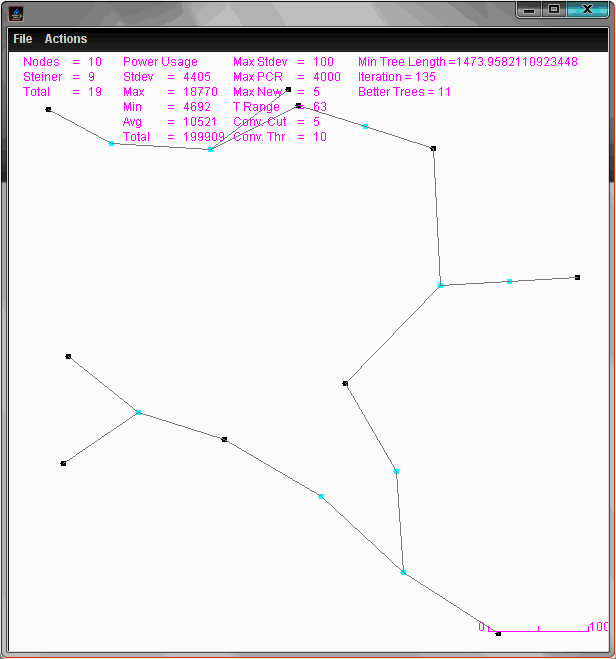
\includegraphics[scale=0.405]{images/1.PNG}
\caption{Steiner Minimum Tree Simulation.}
\label{1}
\end{figure}

A number of configurations were used to collect data.  Varied data elements include every combination of the folllowing:
\begin{itemize}
\item	Canvas size, from 100x100 pixels to 600x600 pixels, increased by increments of 100 
\item	Maximum k value, from 1 to 20 increased by increments of 1
\item	Number of terminal nodes, from 10 to 50, increased by increments of 10
\end{itemize}

Tests were run 10 times each and the results were averaged for more accurate results.  Following are graphs depicting the results, and the group's interpretation of the results.  Although it was mentioned earlier, it is worth repeating that fairness is determined by the standard deviation of the difference between power consumption rates for each node.  Therefore, the more fair a network, the lower the standard deviation. 

\subsection{Results}

Within reach graph, the results are separated according to the size of the canvas on which fairness was measured.  The differences are dramatic as the canvas size increases because the distance between nodes can be much greater.

\subsection{Fairness With Varying Number of Terminal Nodes}

The following three graphs show the total power consumption for different numbers of terminal nodes.  In all three cases, the graphs confirm intuition: as the number of relay nodes increases, the graphs become more fair.  Fairness increases because there are more opportunities to minimize the difference in distances.

\begin{comment}
\begin{figure}[p]
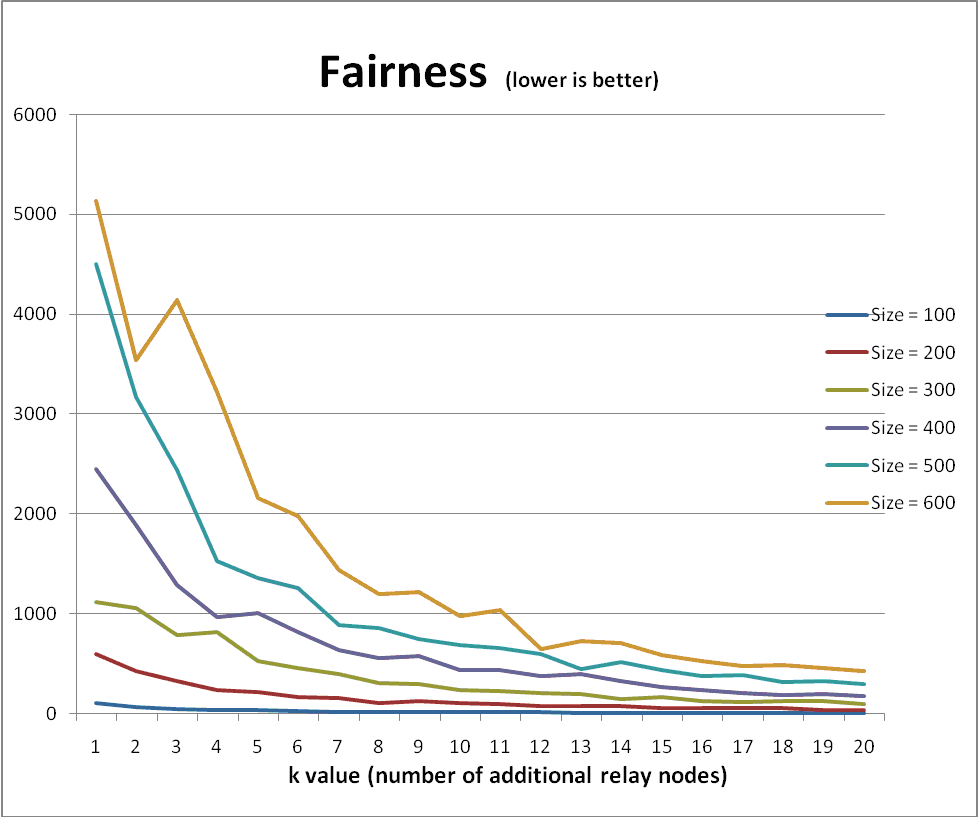
\includegraphics[scale=0.405]{images/2.PNG}
\caption{Fairness as $k$ increases; 10 terminal nodes}
\label{2}
\end{figure}

\begin{figure}[p]
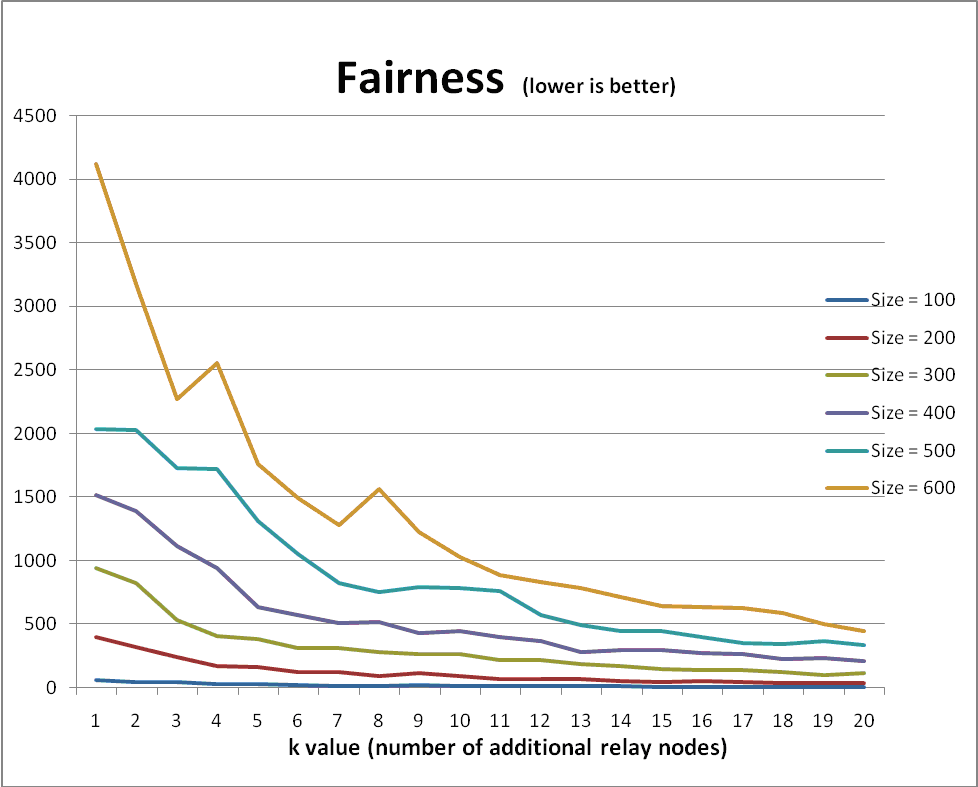
\includegraphics[scale=0.405]{images/3.PNG}
\caption{Fairness as $k$ increases; 20 terminal nodes}
\label{3}
\end{figure}

\begin{figure}[p]
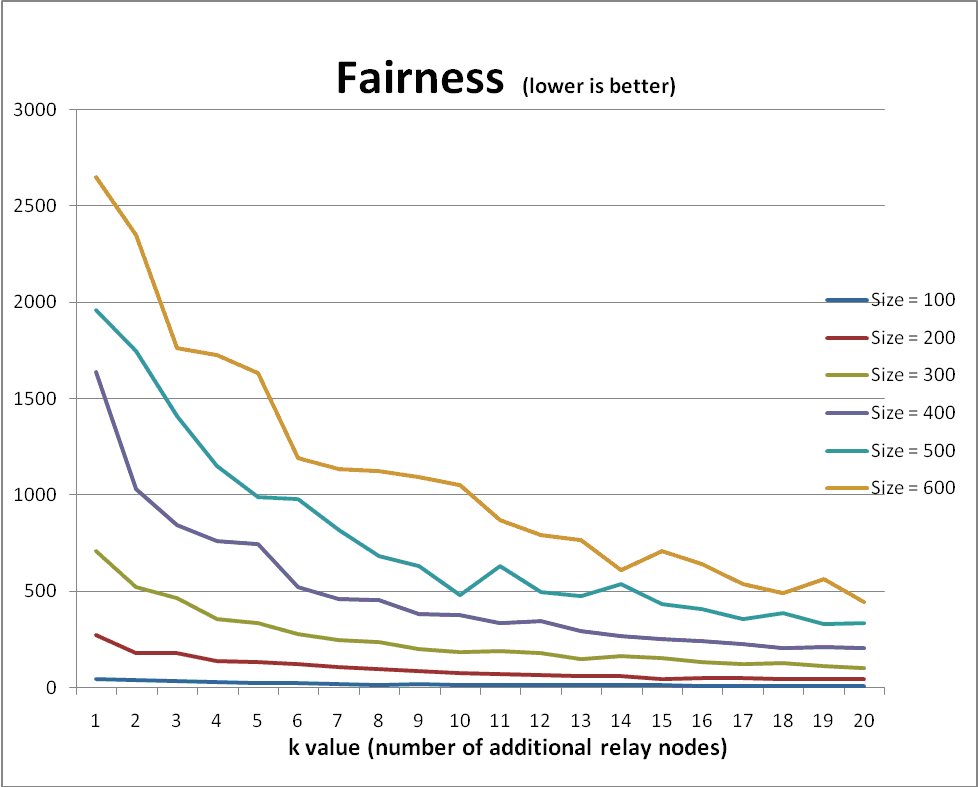
\includegraphics[scale=0.405]{images/4.PNG}
\caption{Fairness as $k$ increases; 30 terminal nodes}
\label{4}
\end{figure}
\end{comment}

Fairness is significantly different for large canvas sizes compared to smaller ones, so in order to better illustrate the trend towards fairness as k increases on small canvases, Figure \ref{5} shows a single canvas size-100x100 pixels-graphed against an increasing k.  As expected, it depicts increasing fairness as the number of relay nodes increases.

\begin{comment}
\begin{figure}[p]
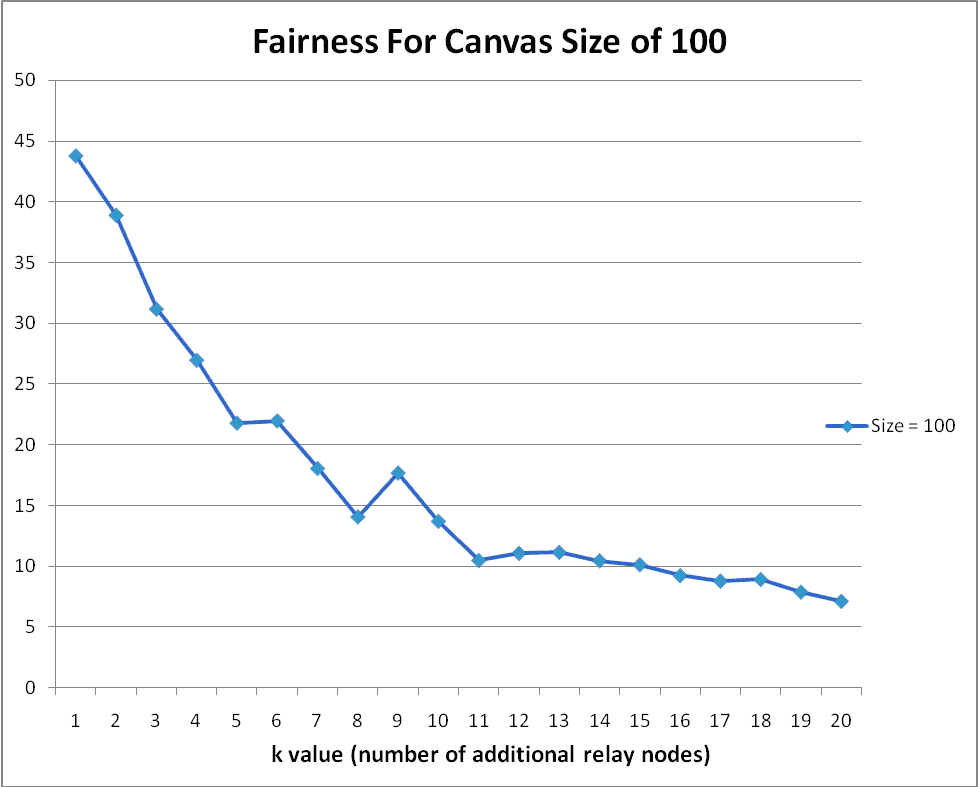
\includegraphics[scale=0.405]{images/5.PNG}
\caption{Fairness as $k$ increases; 30 terminal nodes, and a canvas size of 100x100 pixels.}
\label{5}
\end{figure}
\end{comment}

\subsection{Power Consumption}

Another interesting metric is what happens to the total power consumption as surface area increases.  As explained in an earlier section, the PCR increases as distance between nodes increases.  Power consumption, therefore, decreases based on two factors: as k increases, and as the surface area decreases.  Figure \ref{6} illustrates this. 

\begin{comment}
\begin{figure}[p]
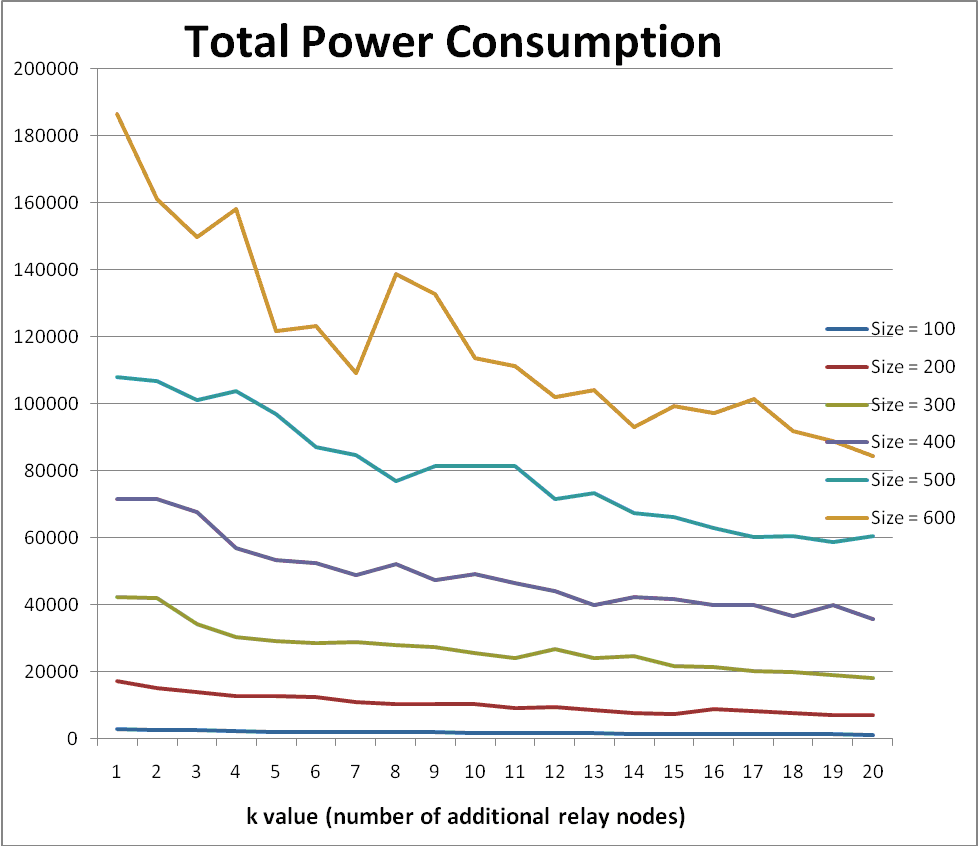
\includegraphics[scale=0.405]{images/6.PNG}
\caption{Total power consumption as $k$ increases; 20 terminal nodes.}
\label{6}
\end{figure}
\end{comment}

Total power consumption, however, is less important in the context of this paper.  More important is fairness.  To illustrate fairness in power consumption, Figure \ref{7} shows the power consumption per node on a 300x300 pixel canvas, with 20 terminal nodes, graphed as k increases.  When k is low, there is little to be done to make the network fair.  By contrast, as k increases, the maximum, average, and minimum power consumption per node start to converge. 

\begin{comment}
\begin{figure}[p]
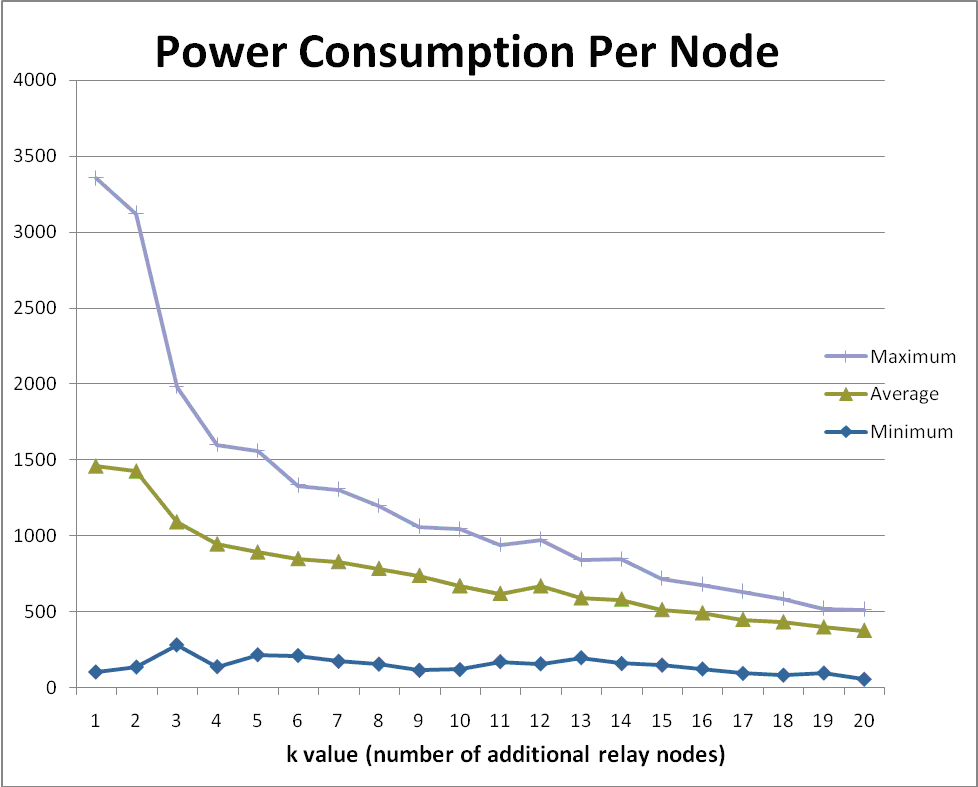
\includegraphics[scale=0.405]{images/7.PNG}
\caption{Power consumption per node on a 300x300 pixel canvas; 20 terminal nodes.}
\label{7}
\end{figure}
\end{comment}

\subsection{Interpretation of Results}

Unfortunately, the authors of this paper could not find literature studying fairness.  Consequently, it is difficult to compare the findings of this paper against some previous standard.  This section, therefore, will not compare its results with other papers.  The results of experimenting, however, do meet expectations: as relay nodes are added, fairness increases.  This is little help ultimately, as it naively implies that k should increase indefinitely.  Clearly this cannot happen: if k approaches some very large number, the sensor network might as well be wired!  The problem, then, is to find a good cutoff for k.

\subsection{Optimal K Value}

Optimal k values change based on the number of terminal nodes and the surface area of the sensor network.  The graphs above and the rest of the data from experimentation show that there are very significant gains in fairness as k increases from 0 regardless of the number of terminal nodes and surface area.   For networks in a small surface area, for example 100x100 to 300x300, fairness shows little gain after k reaches 8 to 12 relay nodes, depending on the number of terminal nodes.  The graphs start to level off earlier when the number of terminal nodes is high, while fewer terminal nodes result in more relay nodes to reach approximate fairness.  Larger surface areas exhibit the same behavior, but require larger k values before leveling off.  Although there isn't a single optimal k value that fits all applications, the important aspect of the fairness is that results tend to be consistent: as k increases, fairness increases, and as surface area decreases, fairness also increases.
The optimal k value, therefore, should be found experimentally, given the practical constraints of the network and application.  For instance, if the surface area of the sensor network is very small, the optimal k value will very likely be lower than a network with double the surface area.

\section{Software Simulation}

The algorithms as described in section \ref{connectingNodes} and \ref{OptimizingNodeLocation} have been implemented and augmented with a graphical user interface (GUI). The GUI allows for the plotting of sensor (shown as white points) and relay nodes (shown as red points) and their corresponding edges in 2D-space. Figure \ref{gui} illustrates the GUI showing a graph of 11 sensor nodes and 10 relay nodes. The graph has been optimized to maximize energy consumption fairness. The GUI supports the loading and saving of nodes. Once a dataset of sensor nodes is loaded, the interface connects the nodes using the Steiner Minimum Tree approximation described in section \ref{connectingNodes}. The \textit{Action} menu item enables control over the fairness optimization algorithms described in section \ref{OptimizingNodeLocation}. The top part of the interface displays statistical information such as total power consumption and fairness in power consumption of the sensor network.

\begin{figure}[ht]
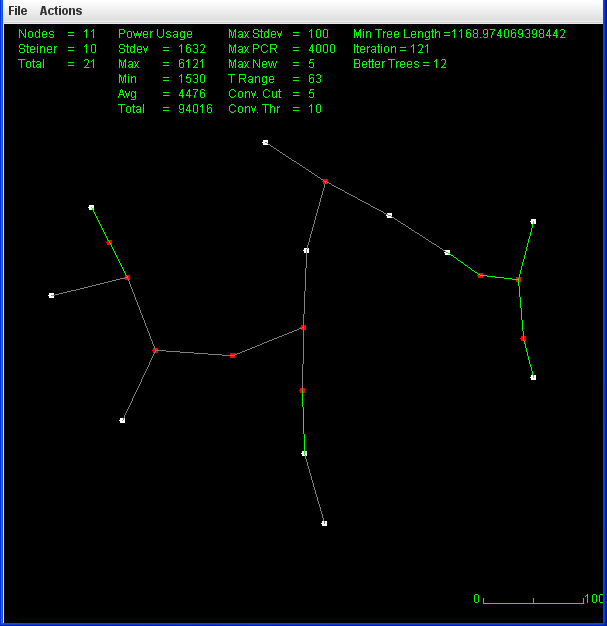
\includegraphics[scale=0.405]{images/graphical-interface.PNG}
\caption{The graphical user interface (GUI) for creating \textit{fair} sensor networks. 11 sensor (white) and 10 Relay (red) nodes are plotted in 2D-space. The image shows the resulting sensor network after optimizing energy consumption fairness.}
\label{gui}
\end{figure}


\section{Conclusion}\label{conclusion}

Approximating fairness in sensor networks has had little to no attention in the literature.  This is perhaps because in many cases, only total power consumption matters.  When dealing with sensor networks where changing, repairing, or working on sensors is invasive-for instance a sensor network on a person, or a network in a difficult to reach destination-fairness becomes important.  As discussed throughout the paper, the reason fairness is important is to ensure node failures occur approximately at the same time.  With approximate fairness, this becomes possible with regard to battery failure, as nodes will deplete power reserves at roughly the same rate.  With node failures occurring at the same time, it allows a network to operate under better-understood and more predictable conditions, as well as helping to avoid two undesirable properties.  First, invasive node replacement procedures do not occur as frequently as if single nodes were allowed to consume power at significantly different rates: with unfair conditions, certain nodes may fail significantly sooner than others, thereby requiring replacement procedures more frequently.  Second, because the procedure is invasive, it is desirable to replace all nodes during the same procedure; under this model, fairness means less waste, since there will be fewer nodes with significant battery power left, while unfair networks potentially waste nodes with significant battery power if all nodes are replaced at the same time.

The fairness approximation procedure discussed above is difficult to measure in any absolute sense.  The reason is twofold: first, there are no baseline comparisons to be made, as the authors could not find fairness studies in the literature; second, and more importantly, the context of the application changes characteristics significantly.  Larger surface areas require more relay nodes to achieve fairness.  Similarly, when the number of terminal nodes is low, more relay nodes are needed to achieve fairness.  Conversely, smaller surface area or more terminal nodes tend to require fewer relay nodes.  These observations are both intuitive and experimentally shown.  This is a significant advantage of the fairness procedure described in this paper: consistent results that follow intuition.  To evaluate the number of relay nodes necessary, it is advisable, therefore, to run simulations and find a $k$ value that best meets the requirements of the application.

\section{Future Work}\label{futureWork}

There are a number of areas touched on in this paper that could be studied more extensively in future work.  The most important consideration that was ignored, which in practical applications will almost definitely be an important measure, is reducing overall power consumption.  The two-fold optimization of optimizing fairness and power consumption would prove very useful in the use cases outlined in this paper, too.

A second future area to consider is connecting all nodes within range and including them in fairness and power measurements.  Currently the algorithm works on a tree without cycles for simplicity, but in any real application of the sensor networks, nodes would need to consider all other nodes within range instead of just one.


\section*{Acknowledgment}

The authors would like to thank Dr. Alan Sherman for his valuable feedback and suggestions related to the design and analysis of the algorithms presented herein and his guidance while writing this manuscript. We are grateful for Neelofer Tamboli for her supporting work regarding this project.



\bibliographystyle{IEEEtran}
\bibliography{IEEEfull,paper}

\onecolumn
\appendix

\begin{figure}[htp]
\centering
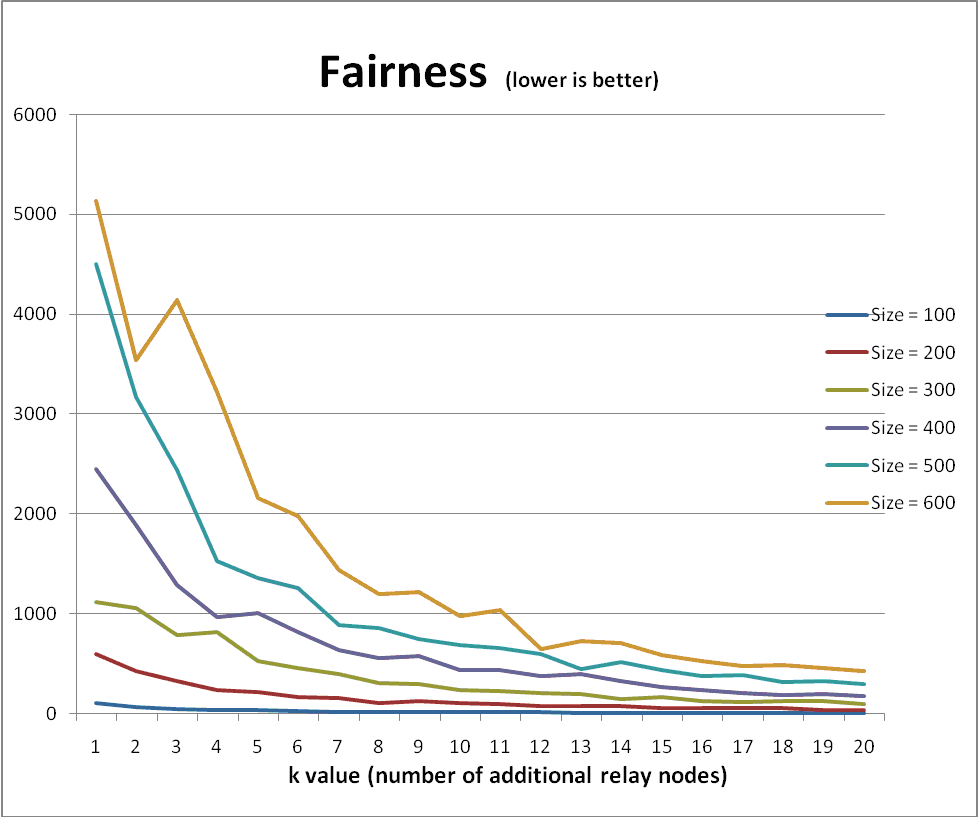
\includegraphics[scale=0.385]{images/2.PNG}
\caption{Fairness as $k$ increases; 10 terminal nodes}
\label{2}
\end{figure}

\begin{figure}[htp]
\centering
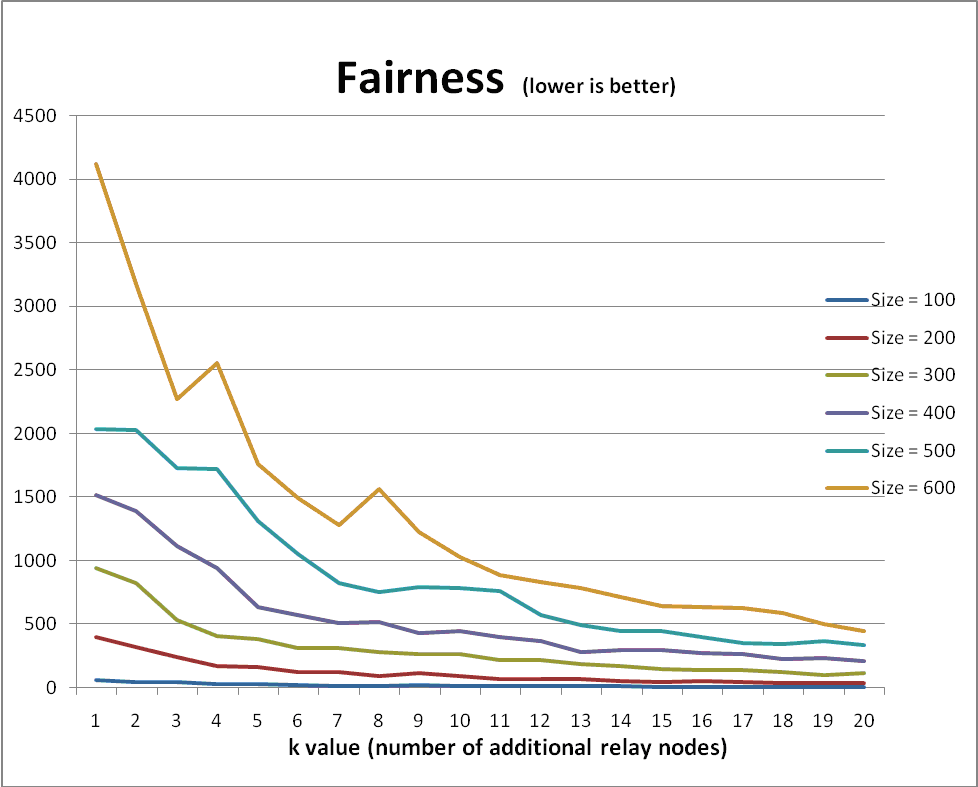
\includegraphics[scale=0.385]{images/3.PNG}
\caption{Fairness as $k$ increases; 20 terminal nodes}
\label{3}
\end{figure}

\begin{figure}[htp]
\centering
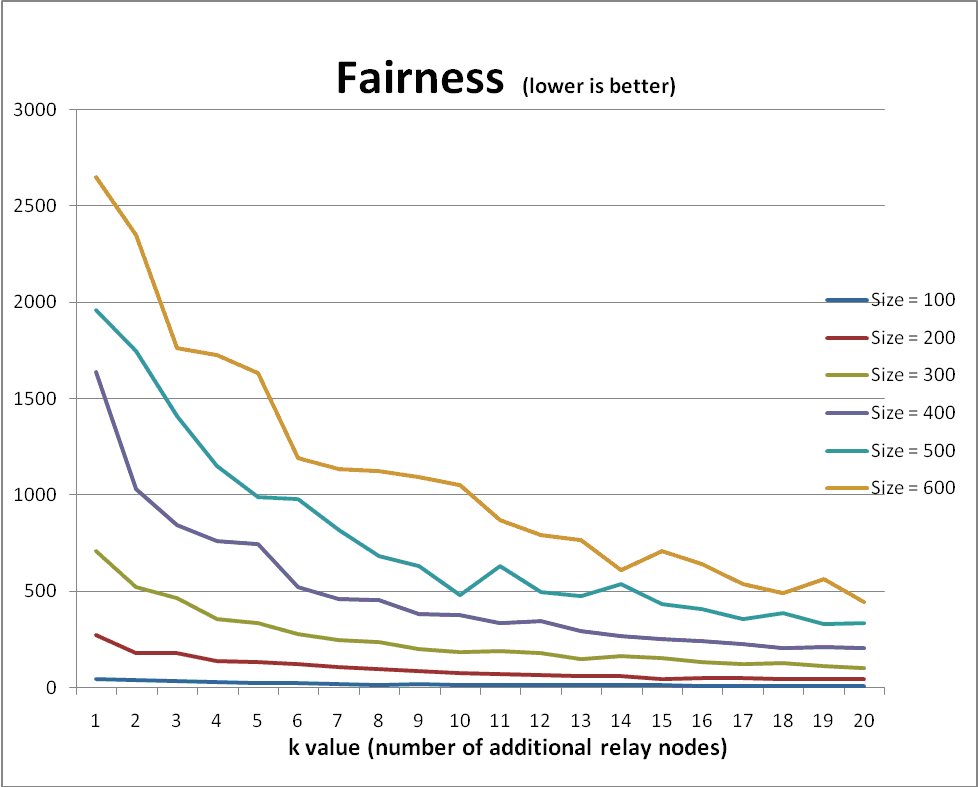
\includegraphics[scale=0.385]{images/4.PNG}
\caption{Fairness as $k$ increases; 30 terminal nodes}
\label{4}
\end{figure}

\begin{figure}[htp]
\centering
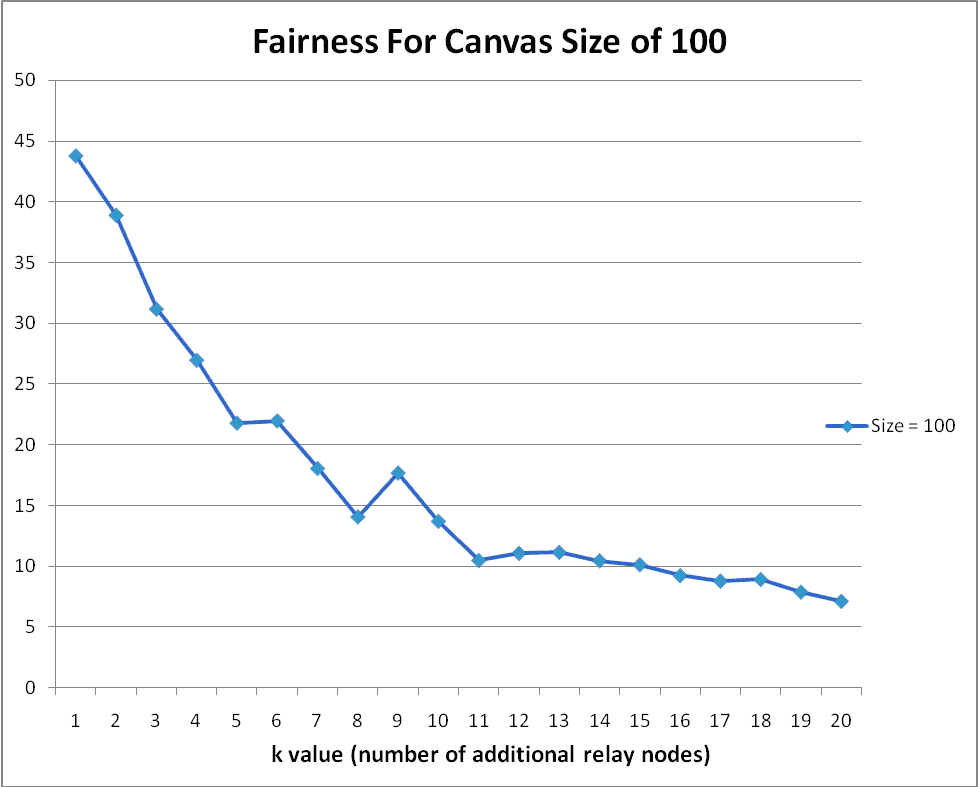
\includegraphics[scale=0.375]{images/5.PNG}
\caption{Fairness as $k$ increases; 30 terminal nodes, and a canvas size of 100x100 pixels.}
\label{5}
\end{figure}

\begin{figure}[htp]
\centering
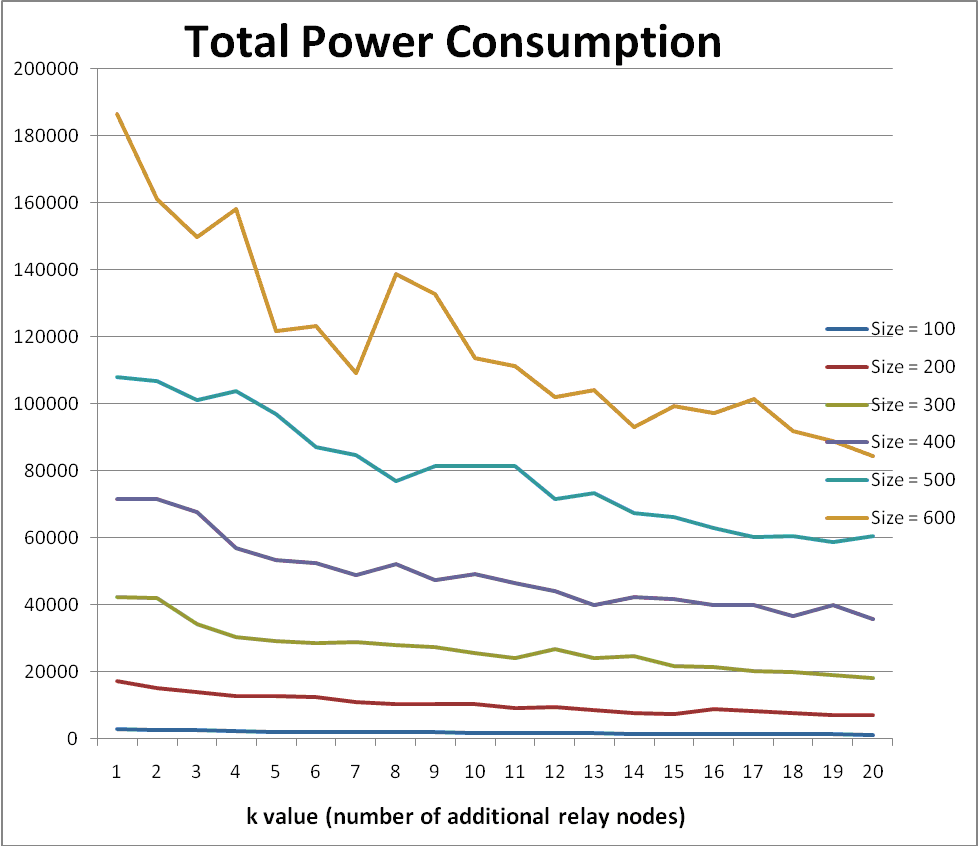
\includegraphics[scale=0.375]{images/6.PNG}
\caption{Total power consumption as $k$ increases; 20 terminal nodes.}
\label{6}
\end{figure}

\begin{figure}[htp]
\centering
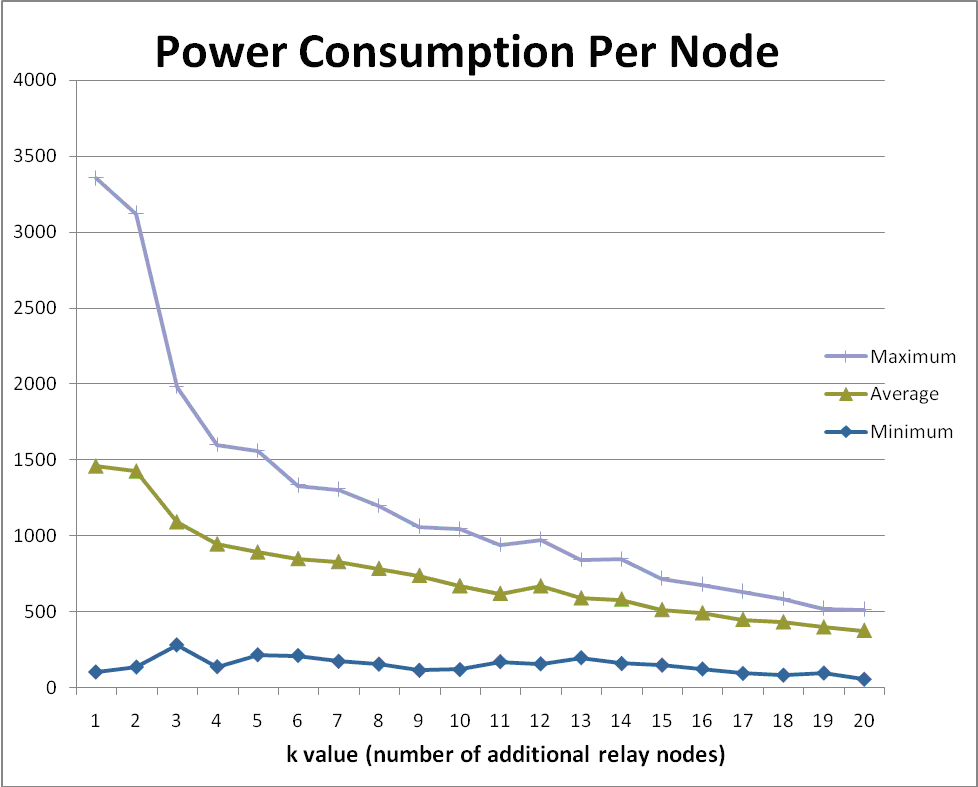
\includegraphics[scale=0.385]{images/7.PNG}
\caption{Power consumption per node on a 300x300 pixel canvas; 20 terminal nodes.}
\label{7}
\end{figure}

% that's all folks
\end{document}



